\documentclass[aspectratio=169]{beamer}
%[handout]

\usetheme[progressbar=frametitle]{metropolis}
\usepackage{appendixnumberbeamer}

\usepackage[utf8]{inputenc}
\usepackage[T1]{fontenc}

\usepackage[brazil]{babel}
\usepackage[outputdir=..]{minted}
\usepackage{xcolor}
\usepackage{soul} % strikethrough
\usepackage{advdate}
\usepackage{graphicx}
\graphicspath{{figs/}}
\usepackage{graphbox}

\usepackage[ampersand]{easylist}

\usepackage{multirow}
\usepackage{multicol}
\usepackage{subcaption}

\usepackage{pgf,tikz}
\usetikzlibrary{shapes,arrows,positioning}
\usetikzlibrary{circuits.logic.US}
\usetikzlibrary{matrix,calc}

\usepackage{karnaugh-map}

\usepackage{pgfpages}
\setbeameroption{hide notes} % Only slides
% \setbeameroption{show only notes} % Only notes
% \setbeameroption{show notes on second screen=right} % Both

% \graphicspath{{../figs/}}

\definecolor{bgc}{rgb}{0.95,0.9,0.95}
\definecolor{links}{HTML}{2A7F7F}
\hypersetup{colorlinks,linkcolor=,urlcolor=links}

\newminted{verilog}{fontsize=\scriptsize, 
    linenos,
    numbersep=8pt,
    bgcolor=bgc,
    tabsize=4,
    framesep=3mm} 
    %frame=lines,

\newcommand{\verilog}[1]{\verilogf{#1}{\footnotesize}}

\newcommand{\verilogf}[2]{\inputminted[fontsize=#2, 
    linenos,
    tabsize=2,
    numbersep=4pt,
    bgcolor=bgc,
    framesep=3mm]{verilog}{../codes/#1.v}
}

\newminted{nasm}{fontsize=\scriptsize, 
		   linenos,
		   numbersep=8pt,
           bgcolor=bgc,
		   framesep=3mm} 

\usepackage{booktabs}
\usepackage[scale=2]{ccicons}

\usepackage{pgfplots}
\usepgfplotslibrary{dateplot}

\usepackage{hyperref}


\usepackage{xspace}
\newcommand{\themename}{\textbf{\textsc{metropolis}}\xspace}



\usepackage{pifont}% http://ctan.org/pkg/pifont
\newcommand{\cmark}{\ding{51}}%
\newcommand{\xmark}{\ding{55}}%

% \tiny	
% \scriptsize
% \footnotesize
% \small	
% \normalsize	
% \large	
% \Large	
% \LARGE	
% \huge	
% \Huge	



\newminted{python}{fontsize=\scriptsize, 
		   linenos,
		   breaklines,
		   numbersep=8pt,
           tabsize=2,
		   framesep=3mm} 
		   
\newminted{verilog}{fontsize=\scriptsize, 
		   linenos,
		   breaklines,
		   numbersep=8pt,
           tabsize=2,
		   framesep=3mm} 
		   




\definecolor{bgc}{rgb}{0.95,0.9,0.95}
\definecolor{links}{HTML}{2A7F7F}
\hypersetup{colorlinks,linkcolor=,urlcolor=links}


% \usepackage[style=apa]{biblatex}
% \addbibresource{mm.bib}


% \author{\large Prof. Ricardo Menotti (\href{mailto:menotti@ufscar.br}{menotti@ufscar.br})}

\newcommand{\newauthor}[2]{
  \parbox{0.50\textwidth}{
    \texorpdfstring
      {
        \centering
        \small #1 \newline
        {\scriptsize{\urlstyle{same}\href{mailto:#2}{#2}\urlstyle{tt}}}
      }
      {#1} \newline
  }
}

\author{
  \newauthor{Prof. Ricardo Menotti}{menotti@ufscar.br}
\and \newauthor{Prof. Luciano de Oliveira Neris}{lneris@ufscar.br}  
%\and \newauthor{Prof. Artino Quintino da Silva Filho}{artino@ufscar.br}
% \and \newauthor{Prof. Maurício Figueiredo}{mauricio@ufscar.br}
% \and \newauthor{Prof. Edilson Kato}{kato@ufscar.br}
% \and \newauthor{Prof. Roberto Inoue}{rsinoue@ufscar.br}
}

\date{Atualizado em: \today}

\institute{\large \textbf{Departamento de Computação} \\
Centro de Ciências Exatas e de Tecnologia \\
Universidade Federal de São Carlos}

\title{Lógica Digital (1001351)}

\titlegraphic{\hfill
\includegraphics[height=1.5cm]{LogoUfscar}}



\subtitle{Introdução às ferramentas CAD} % 

\begin{document}

\begin{frame}
	\titlepage
\end{frame} 

\section{Introdução às ferramentas CAD}

\begin{frame}{\insertsection} % Slide with bullets
	\begin{itemize}
		\item As técnicas vistas até agora podem ser usadas para projetar circuitos relativamente pequenos;
		\item Para projetar grandes circuitos, como os dos computadores atuais, são necessárias ferramentas CAD que automatizam boa parte do processo;
		\item Geralmente, elas são comercializas em pacotes, que possuem uma ferramenta para cada etapa do projeto. 
    \end{itemize}
\end{frame}

\begin{frame}{Projeto inicial (\textit{design entry})} % Slide with bullets
	\begin{itemize}
		\item Feito manualmente, pois requer experiência e intuição; 
		\item Esquemáticos;
		\begin{itemize}
		    \item Projeta-se o circuitos desenhando suas portas lógicas e suas conexões; 
		    \item Impraticável para circuitos grandes; 
		\end{itemize}
		\item Linguagem de Descrição de Hardware (HDL\footnote{Do inglês: \textit{Hardware Description Language}});
		\begin{itemize}
		    \item Similar a uma linguagem de programação, mas descreve o hardware ao invés de um programa; 
		    \item Linguagens proprietárias, abertas e padronizadas (IEEE);
		    \item Oferecem portabilidade e reúso de código;
		    \item VHDL e Verilog são as linguagens mais difundidas; 
		    \item Apesar de serem diferentes, oferecem recursos similares;
		\end{itemize}
		\item Pode ser feito de forma hierárquica. 
    \end{itemize}
\end{frame}

\begin{frame}{VHDL\footnote{Do Inglês: \textit{VHSIC\footnotemark{} Hardware Description Language}}}
    \begin{itemize}
        \item Influenciada pelas linguagens Ada e Pascal; 
        \item Criada pelo DoD (US) em 1983 para documentar CIs, posteriormente usada para simulação e síntese; 
        \item Padronizada pelo IEEE 1076-(1987, 1993, 2000, 2002 e 2008). 
    \end{itemize}
    \footnotetext[3]{Do inglês: \textit{Very High Speed Integrated Circuit}}
\end{frame}

\begin{frame}{Verilog\footnote{Da combinação de \textit{verification} e \textit{logic}}}
    \begin{itemize}
        \item Influenciada pelas linguagens C e Fortran; 
        \item Criada em 1983 pela Cadence para simulação, posteriormente usada para síntese e verificação; 
        \item Padronizada pelo IEEE 1364-(1995, 2001 e 2005);
        \item Incorportada ao SystemVerilog IEEE 1800-(2005, 2009 e 2017).
    \end{itemize}
\end{frame}

\begin{frame}{Síntese (lógica)}
    \begin{itemize}
        \item Geração de um circuito lógico a partir de sua especificação; 
        \item Expressões obtidas inicialmente não são ótimas, pois refletem a especificação; 
        \item Parte importante desse processo é obter circuitos equivalentes melhores; 
        \item Nem sempre o objetivo é reduzir o custo, depende da tecnologia de implementação; 
    \end{itemize}
\end{frame}

\begin{frame}{Simulação funcional}
    \begin{itemize}
        \item A partir das expressões de um circuito, é possível realizar a sua simulação; 
        \item Assume que o circuito será implementado com portas perfeitas, ou seja, ignora o atraso de propagação do sinal elétrico;
        \item O simulador exige que o usuário especifique as entradas a serem testadas e fornece as saídas correspondentes; 
        \item Sua saída normalmente é exibida em diagramas de formas de onda;
        \item Também é possível informar as saídas esperadas para que a ferramenta as verifique automaticamente. 
    \end{itemize}    
\end{frame}

\begin{frame}{Projeto físico}
    \begin{itemize}
        \item Determina exatamente como implementar o circuito em um determinado chip;
        \item Mapeiam um circuito especificado na forma de expressões lógicas para uma realização que faz uso dos recursos disponíveis no chip de destino;
        \item Os recursos não são necessariamente portas simples; 
        \item Determina as conexões que devem ser feitas entre esses recursos para implementar o circuito desejado;
    \end{itemize}
\end{frame}

\begin{frame}{Simulação temporal \textit{(Timing/Gate-level simulation)}}
    \begin{itemize}
        \item Circuitos eletrônicos não podem executar sua função com atraso zero, apresentam um \textbf{atraso de propagação};
        \item Quando as entradas de um circuito mudam, leva certo tempo para que a sua saída seja atualizada corretamente; 
        \item Além disso, há o atraso dos sinais que se propagam pelos fios usados para conectar os elementos; 
        \item O simulador avalia os atrasos esperados para que se possa determinar se o circuito atinge os requisitos de desempenho; 
        \item Se a meta não for atingida, o projetista pode tentar repetir o projeto físico informando novas restrições à ferramenta;
        \item Se isso não for suficiente, o projetista preciasa tentar otimizações na síntese ou mesmo modificar o projeto inicial;
    \end{itemize}    
\end{frame}

\begin{frame}{Implementação}
    \begin{itemize}
        \item Tendo verificado que o circuito projetado atende a todos os requisitos da especificação, o circuito é implementado em um chip real;
        \item Se um chip fabricado sob encomenda for criado para esse projeto, essa etapa será chamada de fabricação;
        \item Se um dispositivo de hardware programável for usado, então este passo é chamado de configuração ou programação.
    \end{itemize}
\end{frame}

\begin{frame}{\insertsection}   \centering
    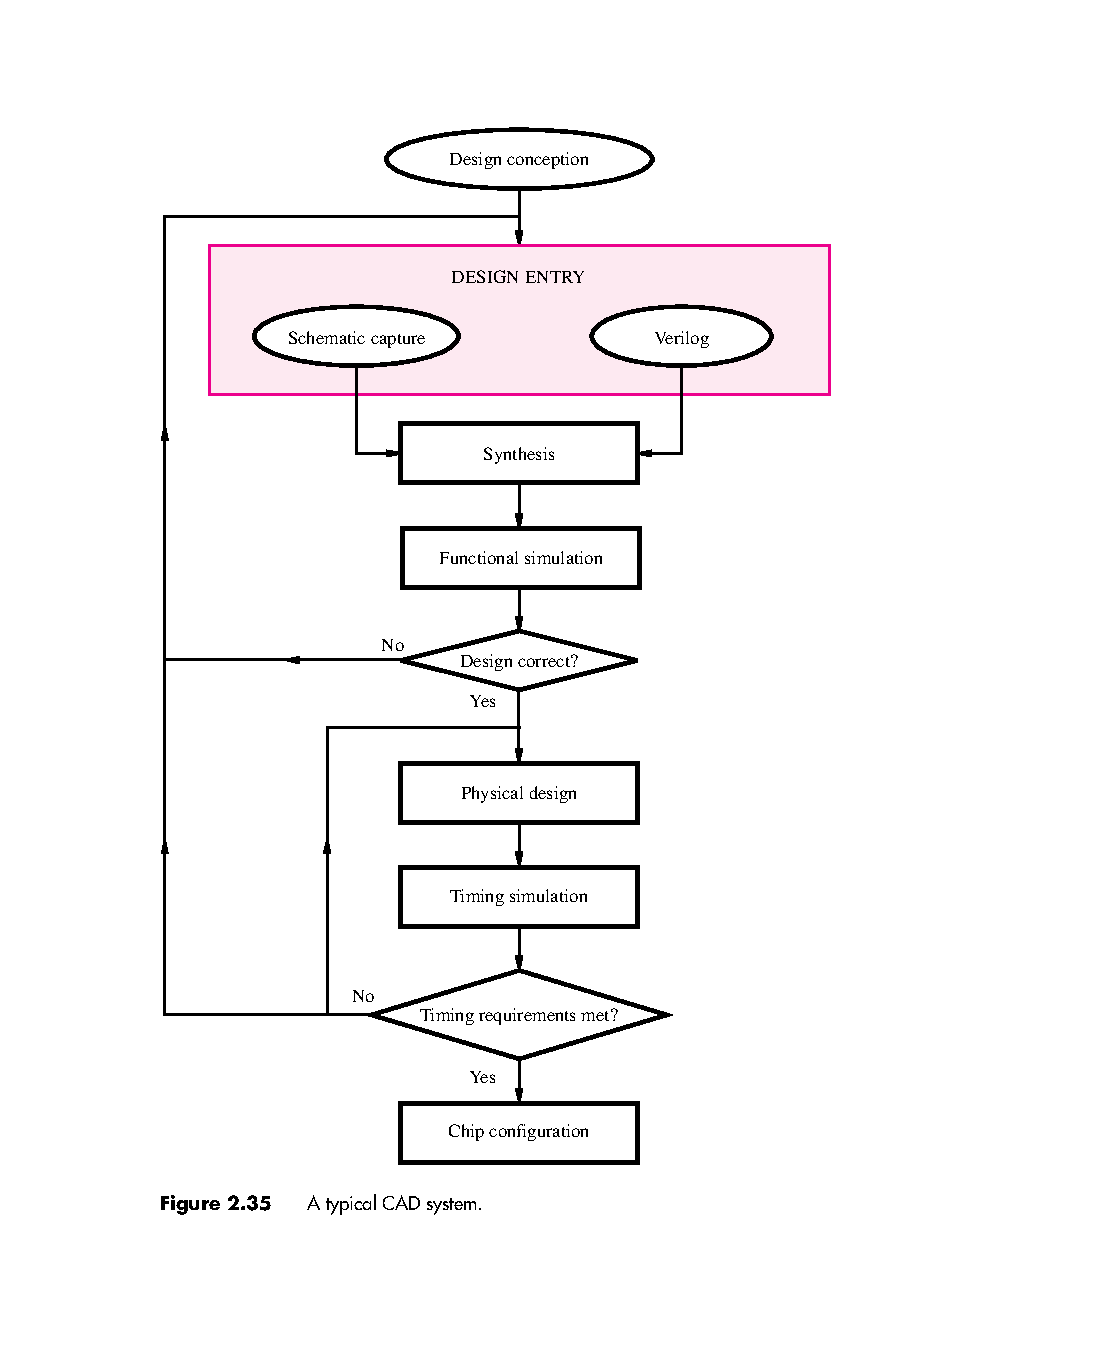
\includegraphics[width=.35\textwidth]{VerilogFig2_35}
\end{frame}

\section{Bibliografia} %%%%%%%

\begin{frame}{\insertsection} 
	\begin{itemize}
		\item \href{https://www.google.com.br/search?q=filetype\%3Apdf+Fundamentals+of+Digital+Logic+with+Verilog+Design+&oq=filetype\%3Apdf}{Brown, S. \& Vranesic, Z. - Fundamentals of Digital Logic with Verilog Design, 3rd Ed., Mc Graw Hill, 2009}
		\item \href{https://en.wikipedia.org/wiki/Template:Programmable_Logic}{Wikipedia Template:Programmable Logic}
	\end{itemize}
\end{frame}

\begin{frame}
	\titlepage
\end{frame} 

\end{document}